% !TeX program = lualatex
% !TeX encoding = utf8
% !TeX spellcheck = uk_UA
% !TeX root =../EMProblems.tex

%=========================================================
\chapter{Випромінювання електромагнітних хвиль}\label{\currfilebase}
\Opensolutionfile{answer}[\currfilebase/\currfilebase-Answers]
\Writetofile{answer}{\protect\section*{\nameref*{\currfilebase}}}%
%=========================================================
%http://www.rec.vsu.ru/rus/ecourse/eldin/izluch.pdf

\section{Електричне дипольне випромінювання}

%{\small 
%
%Потенціали Ліенара — Віхерта:
%
%
%}


%=========================================================
\begin{problem}
Визначити середню повну потужність випромінювання диполя $\vect{p}_e$, що обертається в одній площині з постійною кутовою швидкістю $\omega$.
\begin{solution}
	$I = \frac{2p^2\omega^4}{3c^3}$.
\end{solution}
\end{problem}


%=========================================================
\begin{problem}
Через конденсатор пролетіла частинка з масою $ m $ і зарядом $ q $. Відстань між обкладинками конденсатора $ d $, а напруженість електричного поля $ E $ в ньому однорідне і постійне.
Кут між вектором $ \Efield $ і напрямком швидкості $ \vect{v}_0 $ частинки при вльоті дорівнював $ \alpha $. Знайти енергію, що втрачає частка на дипольне випромінювання під час прольоту через конденсатор.
\begin{solution}
	$W = \frac{2q^3Ev_0}{3mc^3}\left( \sqrt{\frac{2qEd}{mv_0^2}+\cos^2\alpha} - \cos\alpha\right) $.
\end{solution}
\end{problem}

%=========================================================
\begin{problem}
У класичній моделі атома Резерфорда електрон з масою $m$ і зарядом $e$ обертається по коловій орбіті навколо нерухомого ядра з зарядом $Z|e|$. Знайти закон зменшення повної енергії електрона, яке обумовлене дипольним випромінюванням. Обчислити час, після закінчення якого електрон впаде на ядро внаслідок втрати енергії на дипольне випромінювання. У початковий момент часу електрон знаходиться на відстані $R$ від ядра.
\begin{solution}
	$I = \frac{2e^2}{3c^3} \left( \frac{Ze^2}{mR^2}\right)^2 $, $t = \frac{m^2c^3R^3}{4Ze^4}$.
\end{solution}
\end{problem}

\section{Магнітне дипольне випромінювання}

%=========================================================
\begin{problem}
Сила струму круглій рамці в рамці змінюється за законом $I = I_0 \sin\omega t$. Визначити магнітне дипольне випромінювання цієї рамки та повну потужність випромінювання в хвильовій зоні.
%\begin{solution}
%	
%\end{solution}
\end{problem}

%=========================================================
\begin{problem}\label{prb:rad_rotated_ball}
Однорідна куля радіусом $R$ обертається навколо свого діаметра з постійною кутовою швидкістю $\omega$. Вісь обертання нахилена під кутом $\theta$ до напрямку зовнішнього постійного однорідного
магнітного поля $\Bfield$ (рис.~\ref{rad_rotated_ball}). Заряд і маса кулі $q$ і $m$. Визначити інтенсивність випромінювання такої системи.
%---------------------------------------------------------
\begin{figure}[h!]\centering
	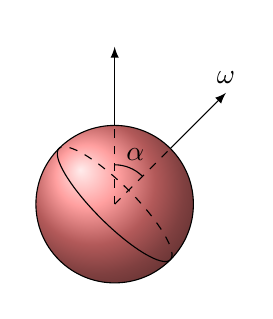
\begin{tikzpicture}
		\begin{scope}[rotate=-45]
			\draw [ball color =red!50] (0,0) circle (1);
			\draw[dashed] (0,0) -- (0,1);
			\draw[-latex] (0,1) -- +(0,1) node[above] {$\omega$};
			\draw (-1,0) arc (-180:0:1 and 0.25) ;
			\draw [dashed] (1,0) arc (0:180:1 and 0.25);
		\end{scope}
		\draw[dashed] (0,0) -- (0,1);
		\draw[-latex] (0,1) -- +(0,1) node[above] {$\Bfield$};
		\draw (0,0.5)  arc (90:45:0.5) node[pos=0.7, above] {$\alpha$};
	\end{tikzpicture}
	\caption{До задачі~\ref{prb:rad_rotated_ball}}
	\label{rad_rotated_ball}
\end{figure}
%---------------------------------------------------------

\begin{solution}
	$I = \frac{q^2\omega^2}{600c} \left( \frac{QBR}{mc^2}\right)^4 \sin^2\theta $.
\end{solution}
\end{problem}

\section{Квадрупольне випромінювання}

%=========================================================
\begin{problem}\label{prb:rad_rotated_disk}
Однорідно заряджений тонкий диск радіусом $R$ обертається навколо свого діаметра з постійною кутовою швидкістю $\omega$. Заряд диска дорівнює $q$. Знайти інтенсивність випромінювання такої системи.
\begin{solution}
	$I = \frac{q^2R^4\omega^6}{10c^5} $.
\end{solution}
\end{problem}

\Closesolutionfile{answer}

